\documentclass{astroedu-lab}

\begin{document}

\pagestyle{plain}

\begin{problem}{\huge Лабораторная работа 5.2.1\\\\Опыт Франка-Герца\\\\Выполнил Жданов Елисей Б01-205}

\section{Цель работы}
Методом электронного возбуждения измерить энергию первого уровня атома гелия в динамическом и статическом режимах

\section{В работе используюются:}
\begin{itemize}
    \item трёхэлектродная лампа ЛМ-2
    \item микроамперметр
    \item понижающий трансформатор
    \item осциллограф
    \item блок источников питания
    \item вольтметр В7-22А
\end{itemize}

\section{Теоретические положения}
Опыт Франка-Герца подтверждает существование дискретных уровней энергии атомов. Разреженный одноатомный газ заполняет трёхэлектродную лампу. Электроны, испускаемые разогретым катодом, ускоряются в постоянном электрическом поле, созданном между катодом и сетчатым анодом лампы. Передвигаясь от катода к аноду, электроны сталкиваются с атомами гелия.
\begin{itemize}
    \item энергия электрона недостаточна, чтобы возбудить/ионизировать атом -> \textit{упругое столкновение}, электрон не теряет энергию
    \item при большой разности потенциалов энергия электрона достаточна для возбуждения атомов -> \textit{неупругое столкновение}, кинетическая энергия передаётся одному из атомных электронов, в результате чего происходит:
    \begin{itemize}
        \item \textbf{возбуждение} - переход одного из атомных электронов на свободный энергетический уровень
        \item \textbf{ионизация} - отрыв электрона от атома 
    \end{itemize}
\end{itemize}

\begin{figure}[h]
\begin{center}
\begin{minipage}[h]{0.45\linewidth}
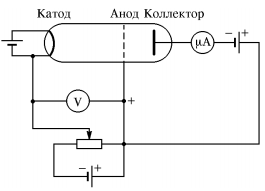
\includegraphics[width=1\linewidth]{fig1.PNG}
\caption{Схема опыта Франка и Герца} %% подпись к рисунку
\label{ris:experimoriginal} %% метка рисунка для ссылки на него
\end{minipage}
\hfill 
\begin{minipage}[h]{0.45\linewidth}
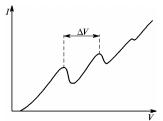
\includegraphics[width=1\linewidth]{fig2.PNG}
\caption{Схематический вид зависимости тока коллектора от напряжения на аноде}
\label{ris:experimcoded}
\end{minipage}
\end{center}
\end{figure}

Объясним вид зависимости тока коллектора (измеряется микроамперметром) от напряжения на аноде. При увеличении потенциала анода ток в лампе растёт и падает (зависимость, подобная ВАХ вакуумного диода). Таким образом, на кривой зависимости тока коллектора от напряжения анода имеется ряд максимумов и минимумов, отстоящих друг от друга на равные расстояния, равные энергии первого возбуждённого состояния.

\newpage

\section{Экспериментальная установка}

\begin{figure}[h]
    \centering
    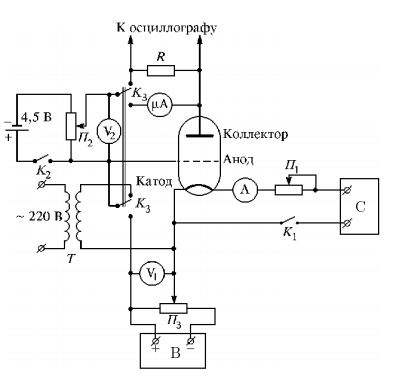
\includegraphics[width=12cm]{fig3.PNG}
    \caption{Схема экспериментальной установки}
    \label{fig:vac}
\end{figure}

\newpage

\section{Измерения, Обработка}

\subsection{Динамический метод}

По результатам, полученным на экране осциллографа получим данные таблицы.

Измерения проводились снятием разницы потенциалов, соответствующих пикам прямого и обратного изменения напряжения, далее эти значения усреднялись и записывались как  $\Delta V_{\max}$ и $\Delta V_{\min}$.
\\
 \begin{table}[h]
 	\centering
 	\begin{tabular}{|l|l|l|l|}
 		\hline
 		$V_{\text{з}}, \;В$ & $\Delta V_{\max}, $ В & $\Delta V_{\min}, $ В & $E,\; \text{эВ}$ \\ \hline
4  & $12\pm 2$   & $19\pm 2$  & $16 \pm 4$     \\ \hline
6  & $10\pm 2$   & $18\pm 2$  & $15 \pm 4$     \\ \hline
8  & $9\pm 2$    & $17\pm 2$  & $14 \pm 4$     \\ \hline
 	\end{tabular}
 \label{tab:1}
 \caption{Результаты динамического измерения}
 \end{table}


Итоговое значение потенциала,
\begin{equation}\label{key}
	E \approx 15 \pm 5 \text{ эВ}
\end{equation}

Погрешности оценены как случайные и соответствующие цене деления шкалы(1 Вольт - малое деление).

\begin{center}
	\Large Осциллограмма $U_\text{задерж} = 8 \text{ Вольт}$
\end{center}

\begin{figure}[!h]
	\centering
	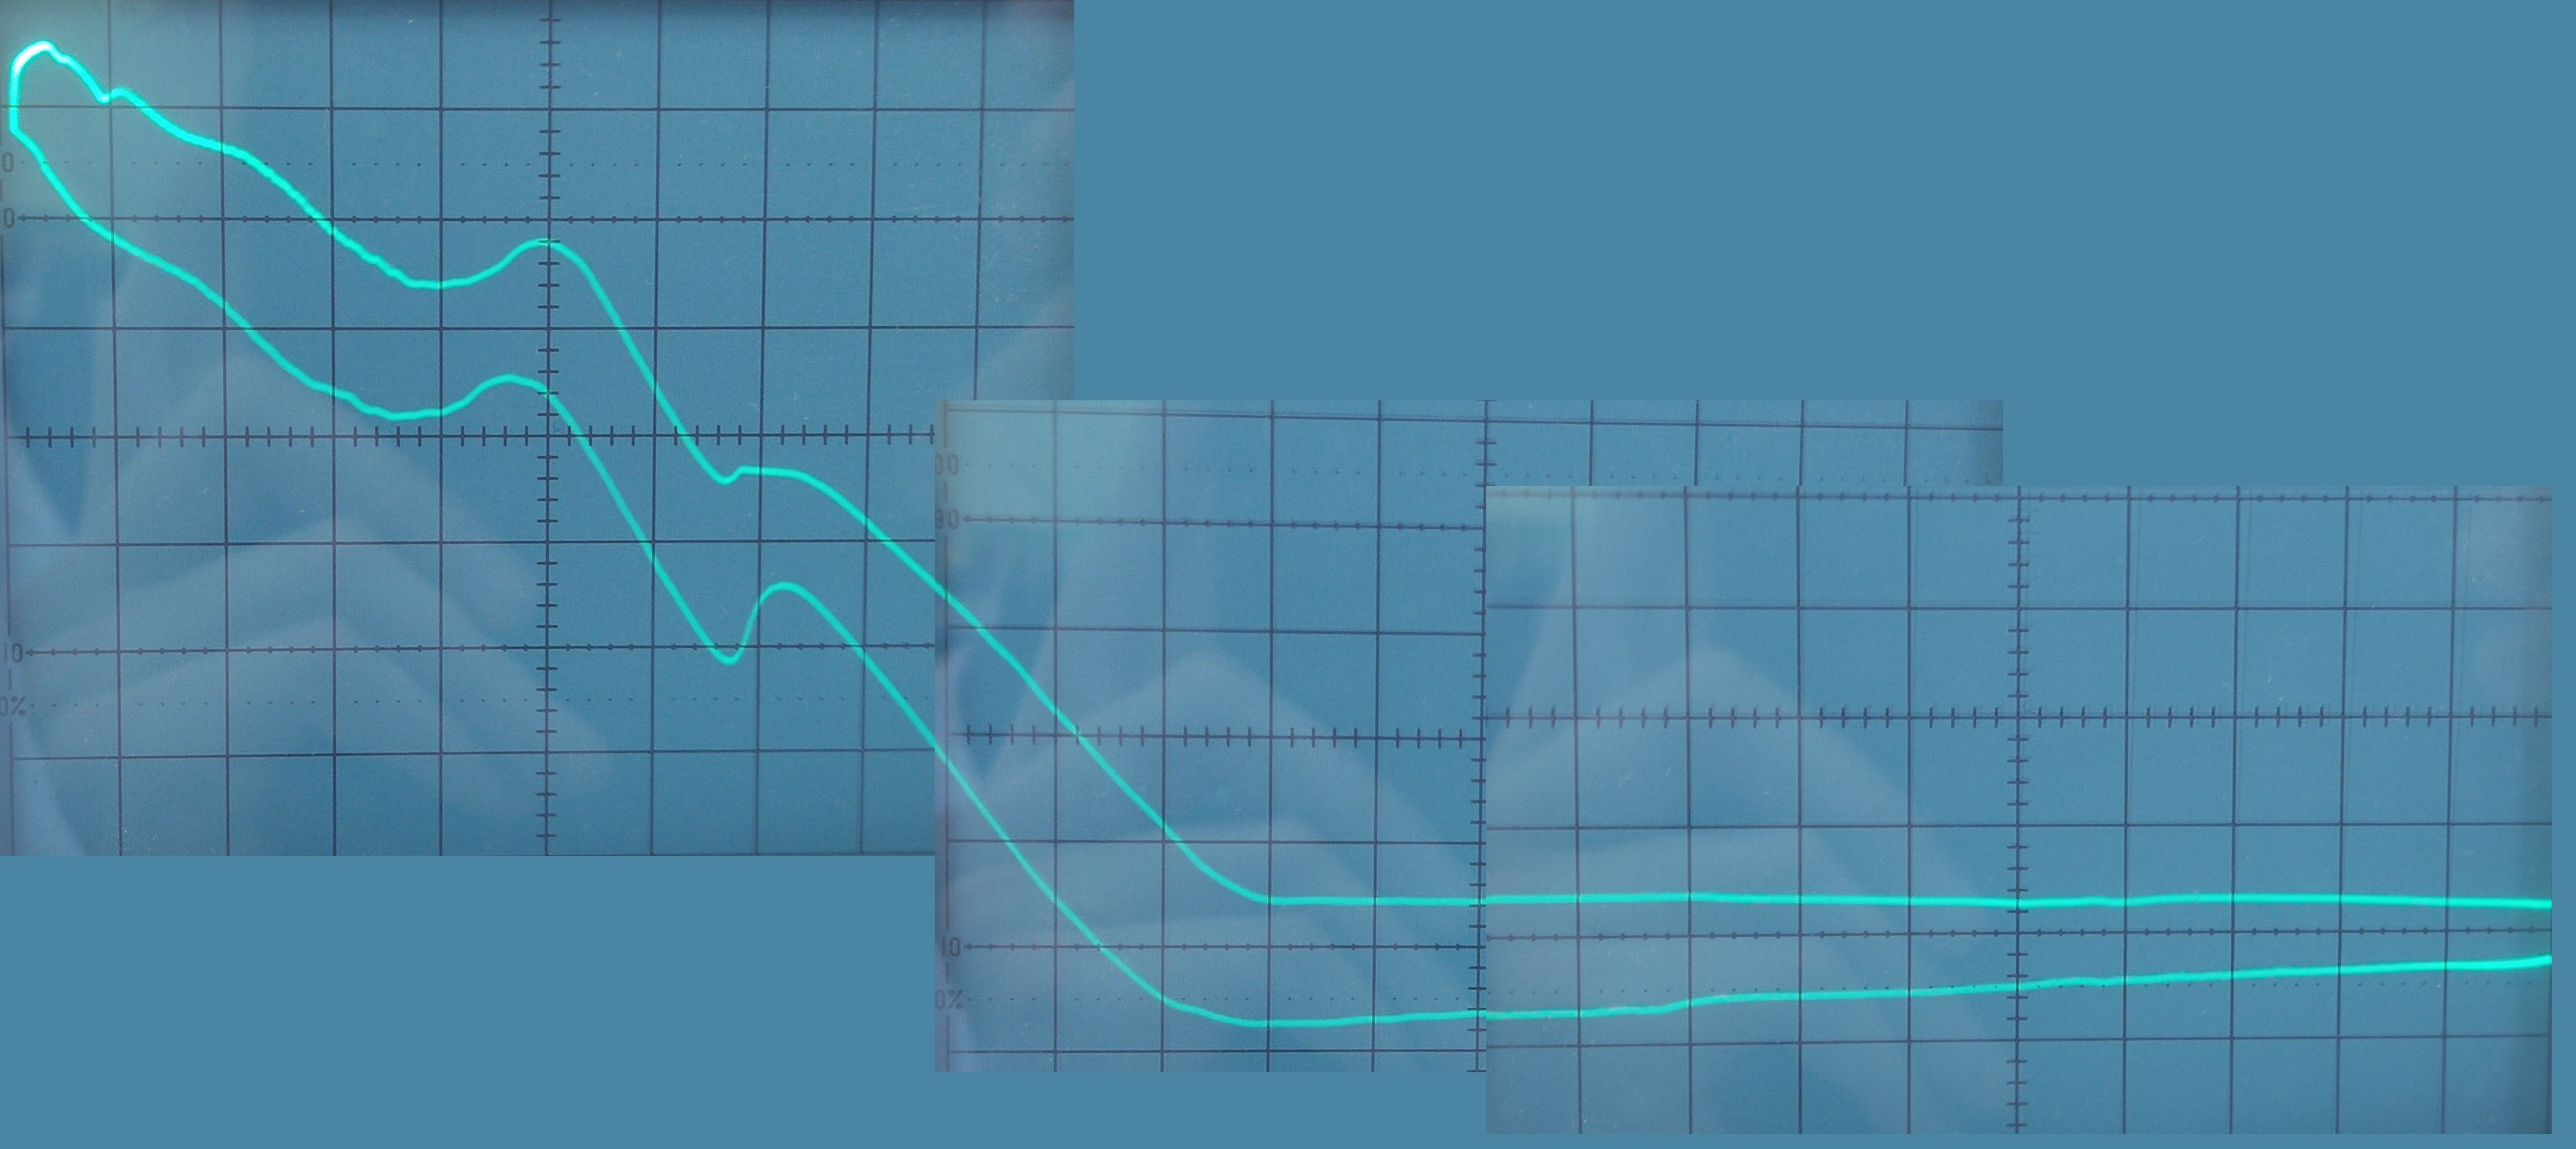
\includegraphics[width=1\textwidth]{8v.jpg}
	\label{fig:boiler}
\end{figure}

%\begin{center}
%	\Large Осциллограмма $U_\text{задерж} = 4 \text{ Вольта}$
%\end{center}
%
%\begin{figure}[!h]
%	\centering
%	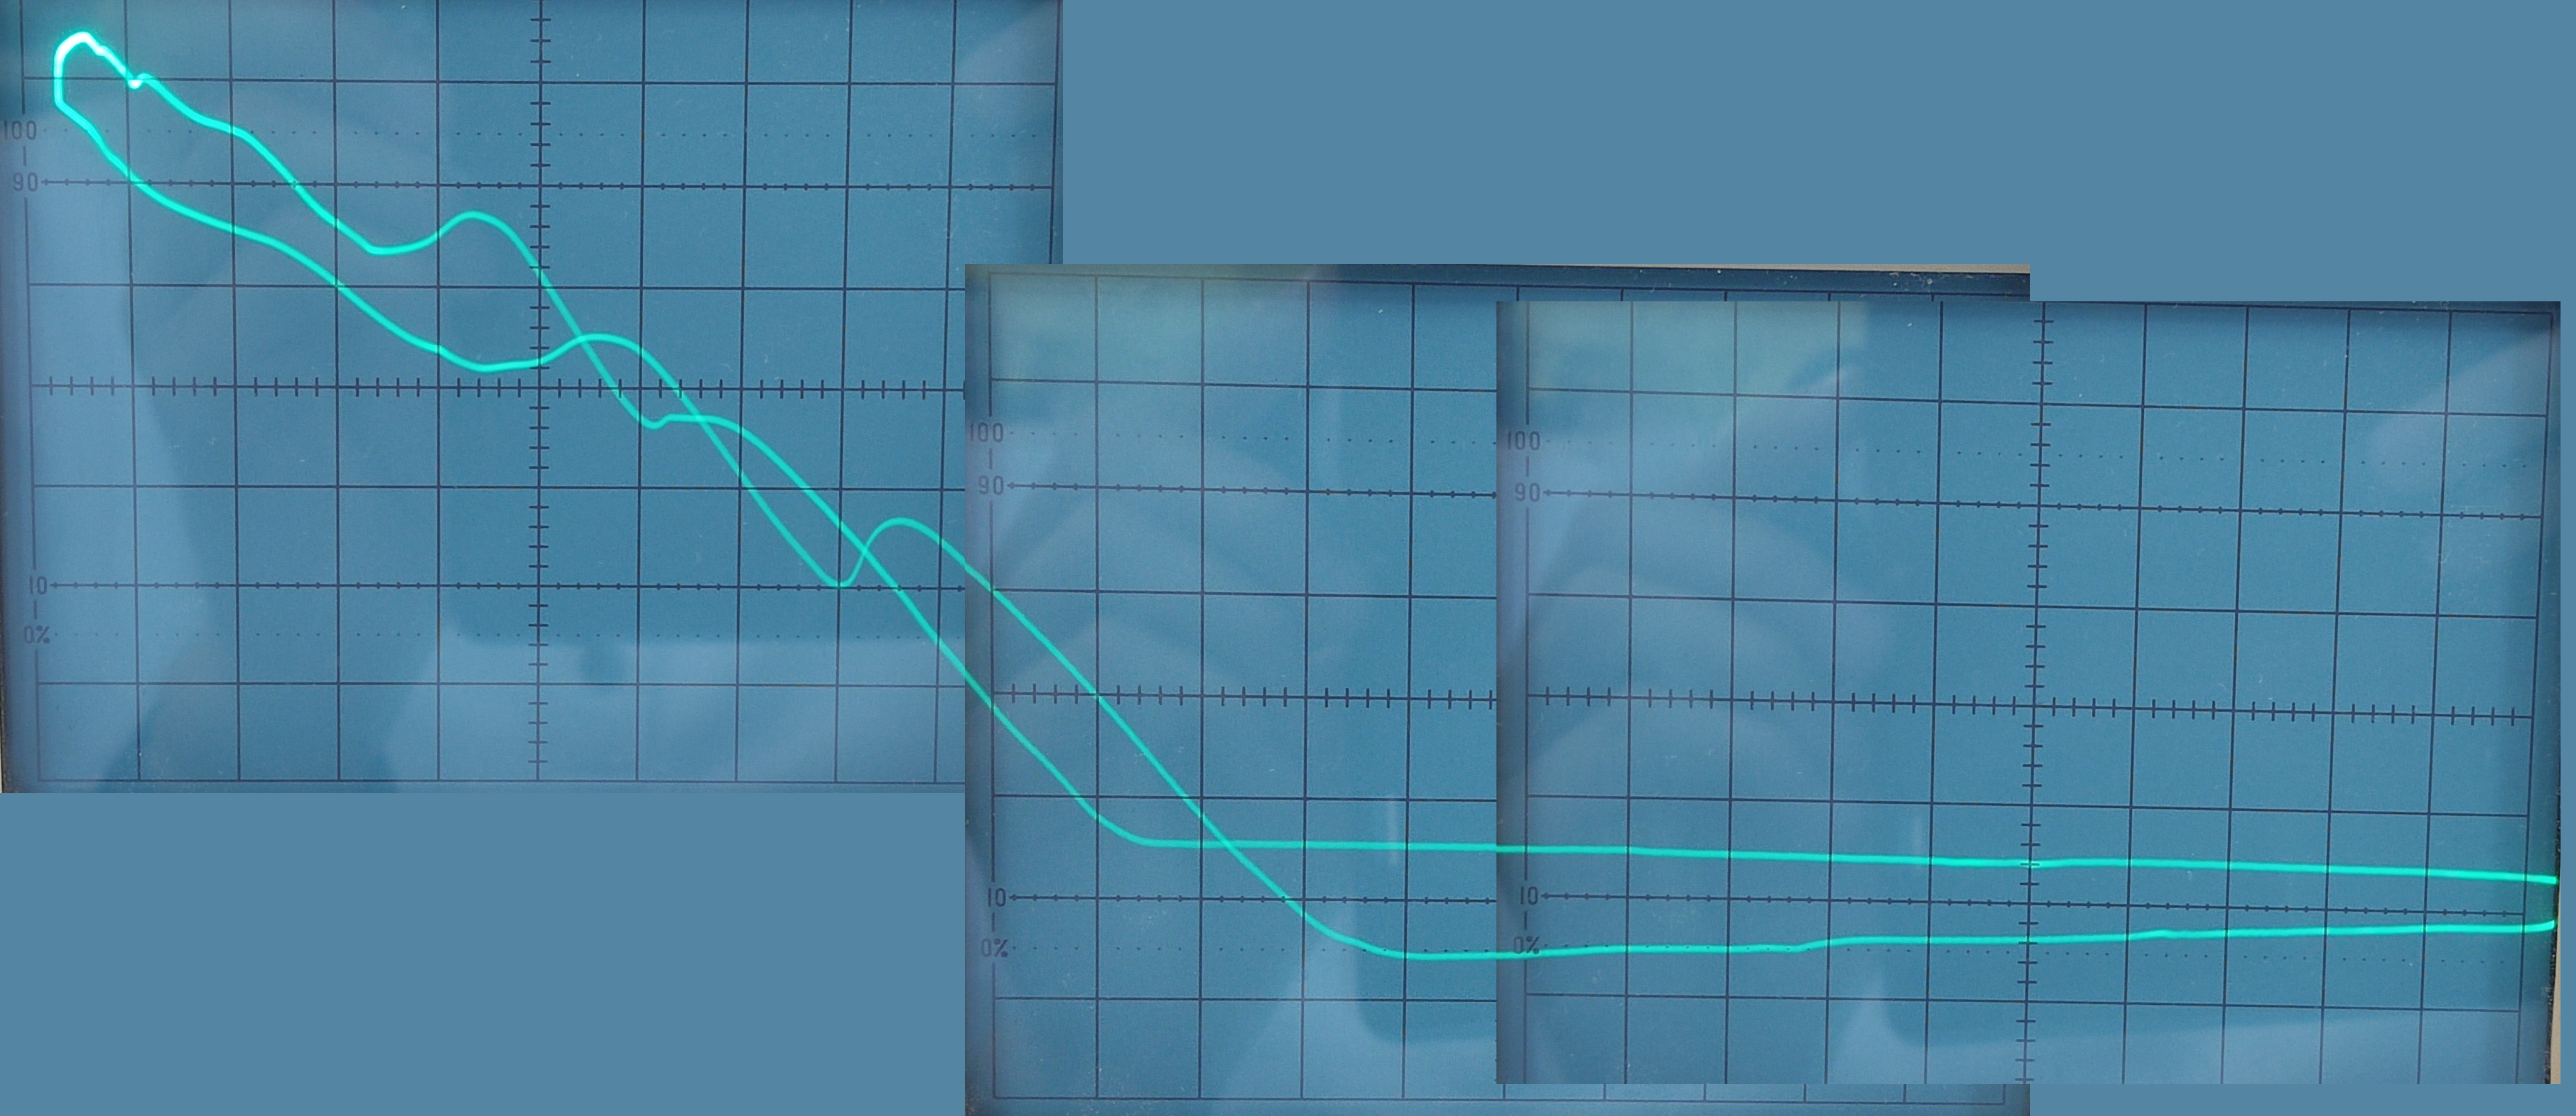
\includegraphics[width=1\textwidth]{4v.jpg}
%	\label{fig:boiler}
%\end{figure}

%\begin{center}
%\begin{tabular}{|c|c|c|c|}
%\hline 
%\multicolumn{2}{|c|}{$h_\text{ман}$, мм} & $\sigma, \frac{\text{мН}}{\text{К}}$ & T, $^\circ$C \\
%\hline
%188.0 & 188.0 & $(64.5 \pm 3.9)$ & 22\\
%187.0 & 187.0 & $(64.0 \pm 3.9)$ & 30\\
%185.5 & 186.0 & $(63.3 \pm 3.9)$ & 35\\
%184.0 & 184.5 & $(62.5 \pm 3.9)$ & 40\\
%182.5 & 183.0 & $(61.7 \pm 3.9)$ & 45\\
%181.0 & 181.0 & $(60.8 \pm 3.8)$ & 50\\
%179.0 & 179.5 & $(59.9 \pm 3.8)$ & 55\\
%177.5 & 177.5 & $(59.0 \pm 3.8)$ & 60\\
%\hline
%\end{tabular}
%\end{center}

\subsection{Статический метод}

Проведем аналогичные измерения в статическом режиме, снимем точки, построим графики и оценим приборные погрешности по характерным осцилляциям напряжений и токов приборов.

 \begin{table}[h]
 	\centering
 	\begin{tabular}{|l|l|l|}
 		\hline
 		$V_{\text{з}}, \;В$ & $\Delta V_{\max}, $ В & $\Delta V_{\min}, $ В \\ \hline
4  & $14.6$   & $20.1$ 			  \\ \hline
6  & $14.1$   & $22.1$       \\ \hline
8  & $14.0$    & $23.5$      \\ \hline
 	\end{tabular}
 \caption{Результаты статических измерений}
 \end{table}
 
Итоговое значение потенциала,
\begin{equation}\label{key}
	E \approx 18 \pm 3 \text{ эВ}
\end{equation}

Погрешность была взята преимущественно случайная, также были учтены погрешности определения максимума и минимума по графикам(порядка 1 Вольта).




%\begin{figure}[!h]
%	\centering
%	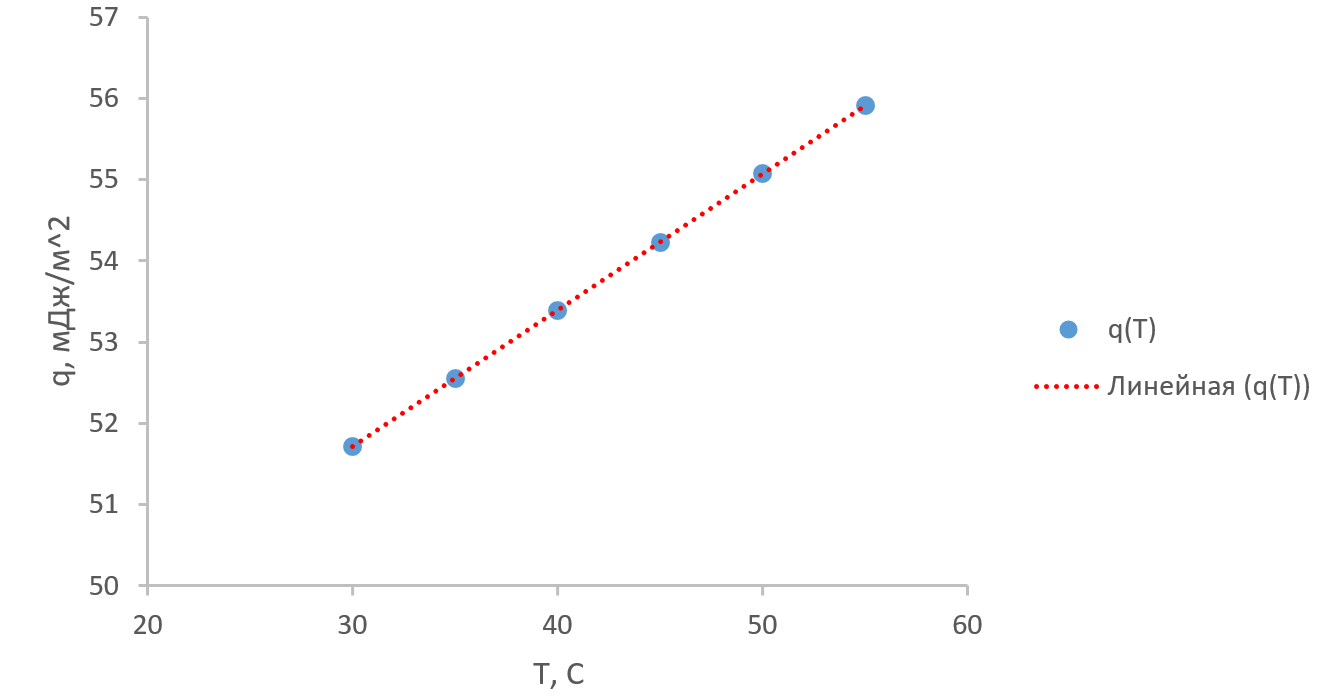
\includegraphics[width=1\textwidth]{2023-02-23_22-23-59.png}
%	\label{fig:boiler}
%\end{figure}

\section{Вывод}

Показания динамического режима: $E \approx 15 \pm 5 \text{ эВ}$

Показания статического режима: $E \approx 18 \pm 3 \text{ эВ}$

Теоретическое значение энергии первого уровня гелия: $E = 21.6$ эВ.

С точностью до погрешности, измеренная величина близка к теоретическому значению, хоть и не дотягивает до него.

Статический метод точнее оценивает значение энергии, вероятно как из-за лучшей точности приборов обработки данных, так и из-за метода рассчетов.


\end{problem}
\end{document}
